\documentclass[conference, harvard, brazil, english]{sbatex}
\usepackage[utf8]{inputenc}
\usepackage{amsmath}
\usepackage{hyperref}
\usepackage{graphicx}
\graphicspath{{images/}}
\usepackage{ae}


\begin{document}
	\title{Projeto Demonstrativo 6 - Reconhecimento de Padrões}
	\date{29-05-2016}
	\author{Samuel Venzi Lima Monteiro de Oliveira\\14/0162241}{samuel.venzi@me.com}
	\address{SQN 208\\Brasília\\Brasil}
		\twocolumn[
			\maketitle
			\selectlanguage{brazil}
		]
	
	\pagenumbering{arabic}
	
	\section{Objetivos}
		\paragraph{}
		Este experimento tem como objetivo realizar estudos de técnicas que permitam implementar algoritmos para análise do processo de reconhecimento de objetos.
		
	\section{Introdução}
		\paragraph{}
		O reconhecimento de padrões tem como objetivo a classificação de objetos dentro de um número de categoria ou classes$^{[1]}$. Para realizar uma classificação, portanto, é necessário o conhecimento das características do objeto de análise, que, por fim, requer que essas características sejam extraídas de alguma forma.
		\paragraph{}
		Pela obra de R. Laganière$ ^{[2]} $, algumas técnicas específicas são eficientes na extração de características de um objeto e seu posterior reconhecimento em outra imagem. Ainda segundo Laganière, o conceito de pontos de interesse ou pontos chave, em visão computacional, se utiliza da ideia que ao invés de olhar uma imagem por completo, pode ser vantajoso selecionar alguns pontos especiais na imagem e realizar uma análise local neles.
		\paragraph{}
		A primeira técnica a ser abordada é a detecção de \textit{Harris corners}. \textit{Corners}, ou esquinas, são uma interessante solução por serem fáceis de localizar em uma imagem e por serem abundantes em grande partes dos casos de reconhecimento. Além disso, são a junção de duas bordas. O OpenCV contém uma função para a detecção de \textit{Harris corners} e a partir dela é possível, com ceta facilidade, melhorar o algoritmo e apresentar uma imagem resultante com as coordenadas das esquinas.
		\paragraph{}
		Outra técnica é a \textit{SURF (Speeded Up Robust Features)}, que introduz a ideia de que cada ponto de interesse deve ter um fator de escala associado. Isso permite com que o objeto ainda seja reconhecido independente da sua escala. Assim como \textit{Harris corner}, o OpenCV cuida da detecção dos pontos chaves, com somente algumas linhas de código. E a partir desses pontos chaves é possível relacioná-los entre duas imagens diferentes e recuperar um resultado de um objeto detectado.
	
	
	\section{Materiais e Metodologia}
		\subsection{Materiais}
			\begin{itemize}
				\item Computador com ambiente Linux (Ubuntu Gnome)
				\item OpenCV
			\end{itemize}
		\subsection{Metodologia}
			\paragraph{}
			O algoritmo de Harris, a fim de definir as esquinas em uma imagem, olha a mudança da intensidade direcional média em uma pequena janela em volta do suposto ponto de interesse.
			\paragraph{}
			\begin{center}
				$ R = \sum (I(x + u, y + v) - I(x,y))^{2} $
			\end{center}
			\paragraph{}
			Onde $ (u, v) $ é um vetor de deslocamento.
			\paragraph{}
			Com manipulações matemáticas, a igualdade acima pode ser transformada em uma aproximação por multiplicação de matrizes, que inclui uma matriz de covariância que caracteriza a variação de intensidade em todas as direções da imagem, computadas utilizando-se operadores de Sobel.
			\paragraph{}
			O OpenCV implementa a função \verb|cv::cornerHarris()| que recupera as esquinas da imagem que pode ser visualizada em uma imagem binária, bastando, posteriormente, realizar melhorias para apresentar os pontos de interesse na imagem original.
			\paragraph{}
			A técnica \textit{SURF} se utiliza da mesma ideia de Harris, porém com a adição do componente de escala.
			\paragraph{}
			Com o objeto \verb|cv::SurfFeatureDetector| pode-se, facilmente, detectar os pontos chave da imagem, e a partir desses pontos e do objeto \verb|cv::SurfDescriptorExtractor|, realizar uma busca do objeto de interesse em uma imagem diferente, posteriormente.
		\section{Resultados}
			\paragraph{}
			Para este experimento, o objeto utilizado foi uma caixa de baralho, por apresentar vários detalhes e permitir uma boa detecção de pontos de interesse.
			\paragraph{}
			\begin{figure}[h]
				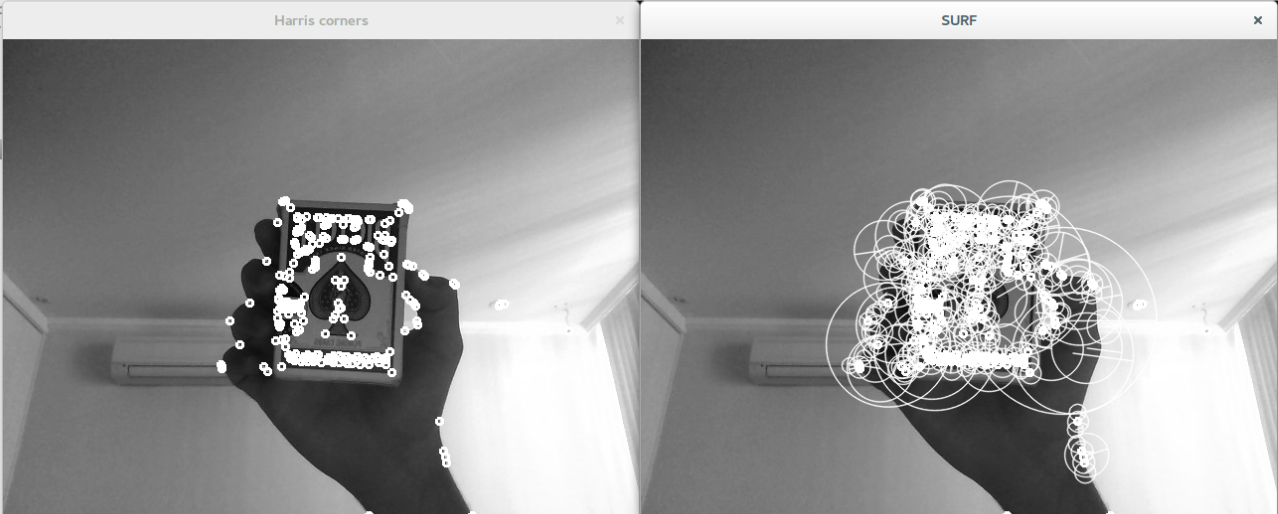
\includegraphics[scale=0.16]{harris-surf}
				\caption{Harris e SURF, lado a lado}
			\end{figure}
			\paragraph{}
			À esquerda, estão os pontos detectador pelo algoritmo de Harris e à direita estão os pontos de interesse detectados pelo algoritmo SURF. 
			\paragraph{}
			Com o algoritmo SURF e a captura de um \textit{template} (neste caso o objeto), a imagem seguinte mostra a relação entre os pontos chave do \textit{template} e os pontos chave encontrados na captura.
			\paragraph{}
			\begin{figure}[h]
				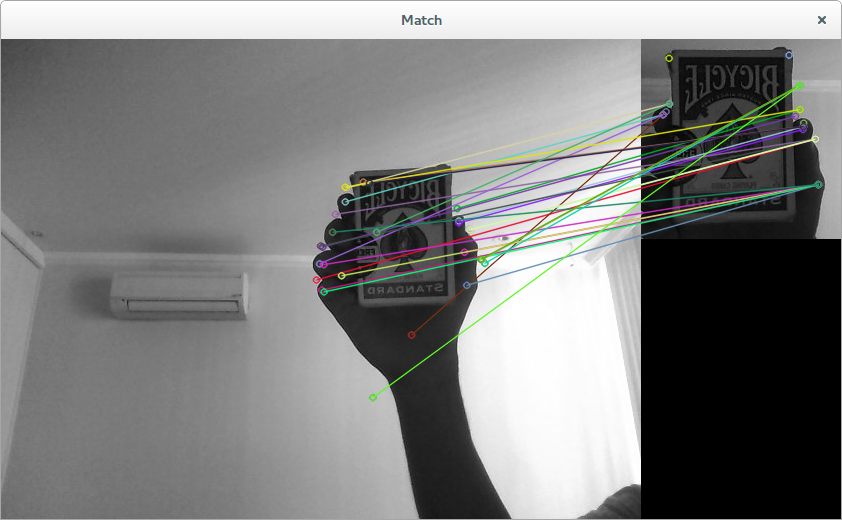
\includegraphics[scale=0.25]{drawmatches}
				\caption{Relação entre \textit{keypoints}}
			\end{figure}
			
			\paragraph{}
			Adaptando o resultado acima é possível realizar o rastreamento do objeto dado que temos o \textit{template} que o representa. Com as coordenadas dos pontos que foram relacionados ao \textit{template} na captura, e uma média simples entre as coordenadas $x$ e $y$ é possível encontrar o centro da zona relacionada (Figura 3).
			\paragraph{}
			\begin{figure}[h]
				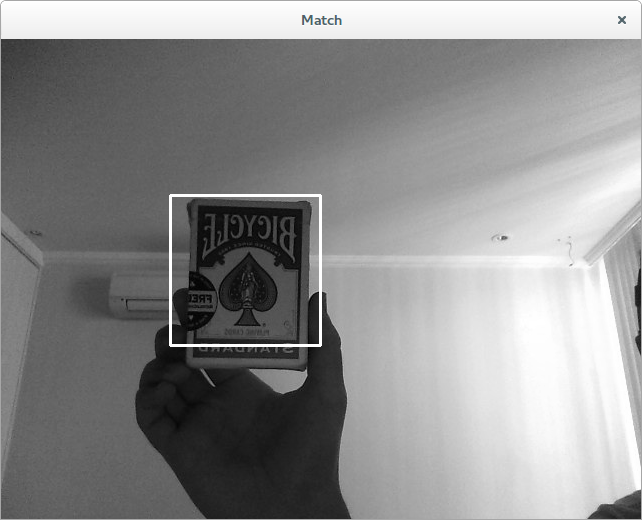
\includegraphics[scale=0.30]{track}
				\caption{Rastreamento}
			\end{figure}
			
		\section{Discussão e Conclusões}
			\paragraph{}
			Na Figura 1, pode-se ver a diferença entre os algoritmos de Harris e SURF, já que SURF, como já dito antes, associa um fator escala a cada ponto de interesse, demonstrado pelas circunferências de raios diversos na imagem. Esse resultado permite relacionar os pontos entre o \textit{template} e a captura (Figura 2).
			\paragraph{}
			Por fim, o resultado da Figura 3 é uma simples adaptação do resultado de \textit{matching} apresentado na Figura 2. Esse resultado é alcançado extraindo a média das coordenadas em $x$ e em $y$ para desenhar o quadrado em volta da coordenada média.
			\paragraph{}
			É importante notar que \verb|SurfFeatureDetector| não disponibiliza nenhuma forma de limitar o número de pontos chave.
			
			\bibliography{bibl}
			\bibliographystyle{harvard}
		\begin{thebibliography}{xx}
			\bibitem{Reconhecimento de padrões} \textit{Pattern Recognition} Sergios Theodoridis, Konstantinos Koutroumbas, 3 ed. Elsevier
			\bibitem{OpenCV2} 
			\textit{OpenCV 2 Computer Vision Application Programming Cookbook} Laganière, R., Packt Pub
			\bibitem{OpenCV documentation}
			\textit{OpenCV Documentation}
			\url{http://docs.opencv.org/2.4.12/}
		\end{thebibliography}
		
		
		
		


\end{document}